\section{MOS Field-Effect Transistors}\label{sec:MOSFETs}
In this section, we start studying \nameref{def:Transistor}s.

\begin{definition}[Transistor]\label{def:Transistor}
  A \emph{transistor} is a \nameref{def:Semiconductor} device used to amplify or switch electronic signals and electrical power.
  Transistors are one of the basic building blocks of modern electronics.
  It is composed of semiconductor material usually with at least three terminals for connection to an external circuit.
\end{definition}

The \nameref{def:MOSFET} is the first \nameref{def:Transistor} we will be studying in this course.
It is the second oldest transistor, but is the most frequently used one today, particularly for digital applications.

\begin{definition}[MOSFET]\label{def:MOSFET}
  \emph{MOSFET}, short for \emph{Metal-Oxide-\nameref{def:Semiconductor} Field-Effect \nameref{def:Transistor}}, is an insulated-gate field-effect transistor.

  The insulated-gate portion of its name implies that the gate is completely isolated from the rest of the circuit.
  This is achieved with the metal oxide layer (seen in \Cref{fig:MOSFET-Physical_Structure-Cross_Section}) acting as an insulator, preventing any current from entering the transistor from that terminal.

  The field-effect portion of the name implies that the electric field of the gate is the driving force in this circuit.
  Because no current is allowed through the gate terminal of the transistor, this only has a voltage applied, causing an electric field to form.

  The typical circuit symbol (for \nameref{def:NMOS}) is shown in \Cref{fig:MOSFET-Symbol-NMOS}.
\end{definition}

The physical structure of a \nameref{def:MOSFET} is shown in \Cref{fig:MOSFET-Physical_Structure-Perspective,fig:MOSFET-Physical_Structure-Cross_Section}.

\begin{figure}[h!tbp]
  \centering
  \begin{subfigure}[h!tbp]{0.48\linewidth}
    \centering
    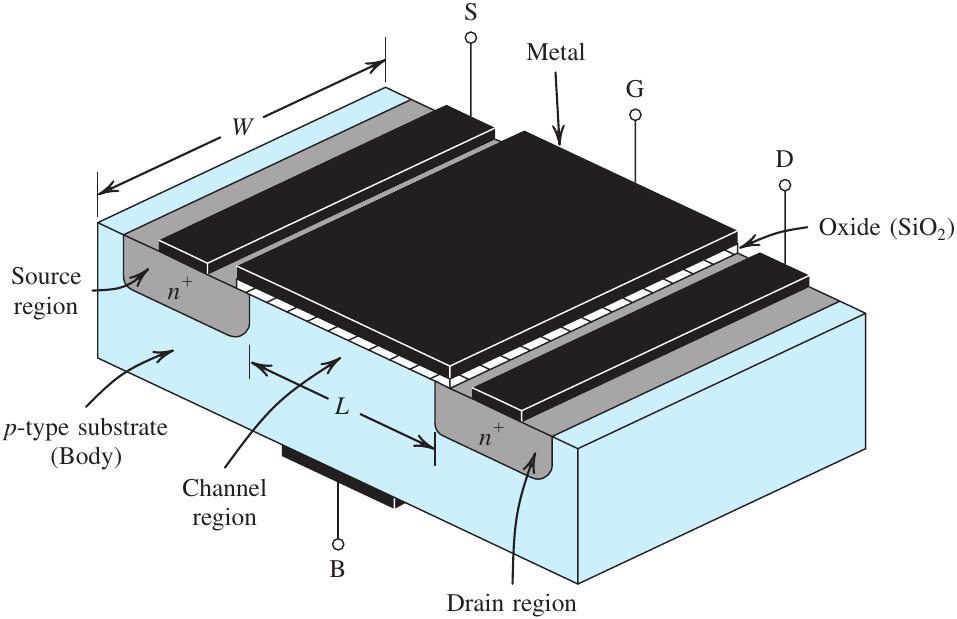
\includegraphics[scale=0.35]{./MOSFET-Physical_Structure-Perspective.png}
    \caption{Perspective View \parencite[p.~249]{sedraTextbook7}}
    \label{fig:MOSFET-Physical_Structure-Perspective}
  \end{subfigure}
  \begin{subfigure}[h!tbp]{0.48\linewidth}
    \centering
    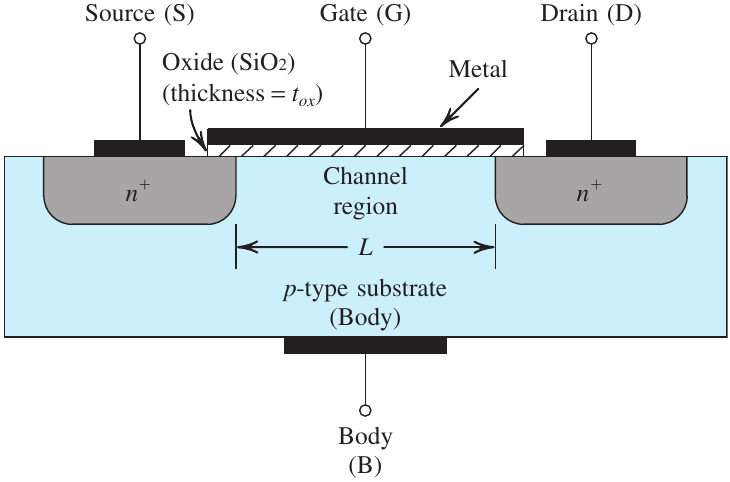
\includegraphics[scale=0.35]{./MOSFET-Physical_Structure-Cross_Section.png}
    \caption{Cross-Sectional View \parencite[p.~249]{sedraTextbook7}}
    \label{fig:MOSFET-Physical_Structure-Cross_Section}
  \end{subfigure}
  \caption{Physical Structure of Enhancement-type \nameref*{def:NMOS} \nameref*{def:Transistor}}
  \label{fig:MOSFET-Physical_Structure}
\end{figure}

As can be seen in \Cref{fig:MOSFET-Physical_Structure-Perspective}, the drain and source both form a \PNJunction{} with the base.

\subsection{No Gate Voltage}\label{subsec:MOSFET-No_Gate_Voltage}
When the gate has \textbf{no} voltage applied, the \PNJunction{}s of the source and drain to the substrate forms a diode-like relationship, where the resistance is very high (of the order $10^{12}\si{\ohm}$)
This prevents nearly all current from the drain from flowing.

\subsection{Gate Voltage Applied}\label{subsec:MOSFET-Gate_Voltage_Applied}
When the gate receives a positive voltage (in relation to the source), then an electric field is formed on the gate, causing a \nameref{def:Depletion_Layer} to form in the substrate.
Then, there is a channel that is formed due to the application of the electric field that allows current to flow between the drain and the source.
\Cref{fig:MOSFET-Gate_Voltage_Applied} shows this phenomena for \nameref{def:NMOS} \nameref{def:Transistor}s.

\begin{figure}[h!tbp]
  \centering
  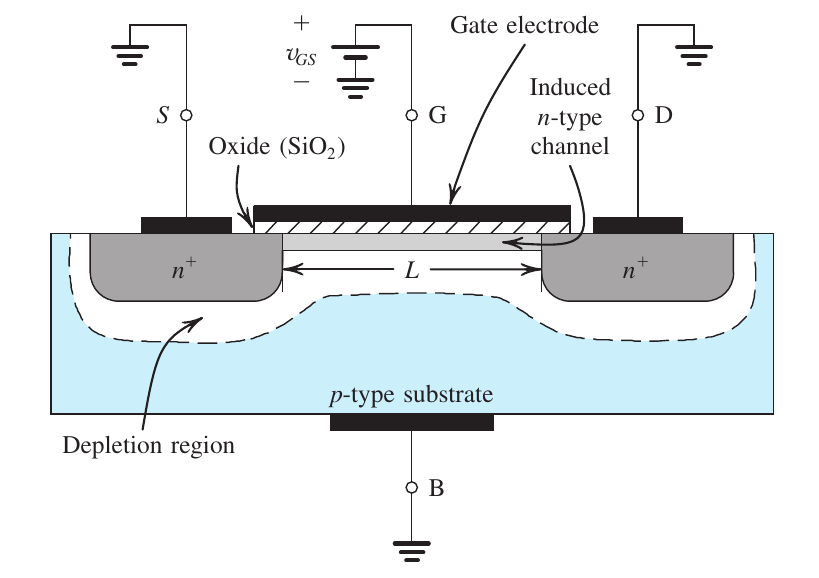
\includegraphics[scale=0.55]{./MOSFET-NMOS-Channel_Created.png}
  \caption{\nameref*{def:NMOS} \nameref*{def:MOSFET} with Positive Voltage Applied to Gate \parencite[p.~251]{sedraTextbook7}}
  \label{fig:MOSFET-Gate_Voltage_Applied}
\end{figure}

\begin{definition}[NMOS]\label{def:NMOS}
  \emph{NMOS}, short for \emph{\Channel{n} Metal-Oxide \nameref{def:Semiconductor}}.
  An \Channel{n} \nameref{def:MOSFET} is formed in a \PType{} substrate, and the induced channel is of \PType{}.
  The channel is created by inverting the substrate surface from \PType{} to \NType{}.
  Hence the induced channel is also called an \emph{inversion layer}.

  The circuit symbol for an NMOS transistor is shown in \Cref{fig:MOSFET-Symbol-NMOS}.
\end{definition}

\begin{figure}[h!tbp]
  \centering
  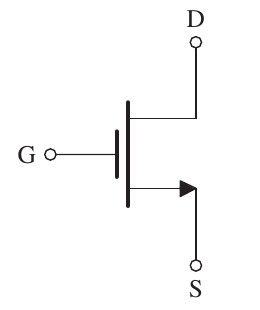
\includegraphics[scale=0.75]{./MOSFET-Symbol-NMOS.png}
  \caption{\nameref*{def:NMOS} \nameref*{def:MOSFET} Circuit Symbol \parencite[p.~265]{sedraTextbook7}}
  \label{fig:MOSFET-Symbol-NMOS}
\end{figure}

\begin{definition}[PMOS]\label{def:PMOS}
  \emph{PMOS}, short for \emph{\Channel{p} Metal-Oxide \nameref{def:Semiconductor}}.
  An \Channel{p} \nameref{def:MOSFET} is formed in a \NType{} substrate, and the induced channel is of \PType{}.
  The channel is created by inverting the substrate surface from \NType{} to \PType{}.
  Hence the induced channel is also called an \emph{inversion layer}.

  The circuit symbol for a PMOS transistor is shown in \Cref{fig:MOSFET-Symbol-PMOS}.
  The physical structure of the PMOS transistor (\Cref{fig:MOSFET-Physical_Structure-PMOS}) is similar to the \nameref{def:NMOS}, which we have studied.
\end{definition}

\begin{figure}[h!tbp]
  \centering
  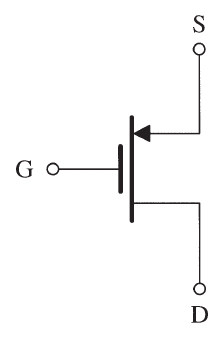
\includegraphics[scale=0.75]{./MOSFET-Symbol-PMOS.png}
  \caption{\nameref*{def:PMOS} \nameref*{def:MOSFET} Circuit Symbols \parencite[p.274]{sedraTextbook7}}
  \label{fig:MOSFET-Symbol-PMOS}
\end{figure}

\begin{figure}[h!tbp]
  \centering
  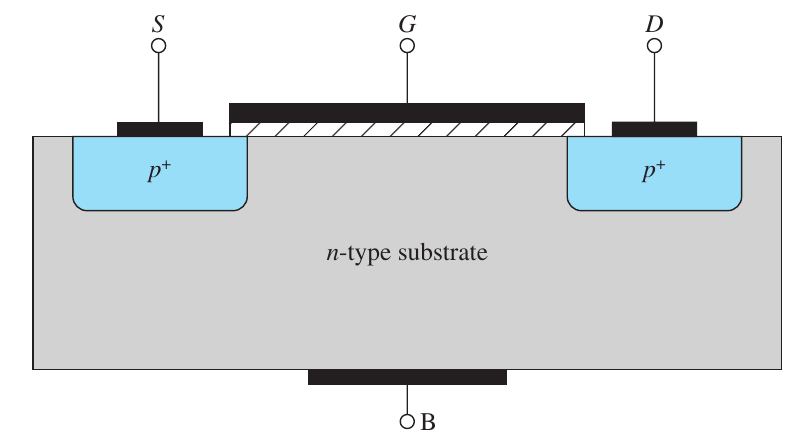
\includegraphics[scale=0.55]{./MOSFET-PMOS-Physical_Structure}
  \caption{\nameref*{def:PMOS} Physical Structure \parencite[p.~262]{sedraTextbook7}}
  \label{fig:MOSFET-Physical_Structure-PMOS}
\end{figure}

For such a channel to form, the voltage between the gate and the source, $\ACVoltage{\Gate\Source}$, \textbf{must} be greater than some \nameref{def:Threshold_Voltage}.

\begin{definition}[Threshold Voltage]\label{def:Threshold_Voltage}
  The \emph{threshold voltage} is a specific value for a \nameref{def:MOSFET} that determines the minimum required forltage that must be aplied at the gate for the transistor to operate.
  In this text, the threshold voltage is denoted as $\ThresholdVoltage$.

  \begin{remark}[Notation]
    Some materials use $\DCVoltage{T}$ as the \nameref{def:Threshold_Voltage}.
    We use $\ThresholdVoltage$, to distinguish this value from the \nameref{def:Thermal_Voltage}.
  \end{remark}
\end{definition}

If the gate-source voltage ($\ACVoltage{\Gate\Source}$) exceeds the \nameref{def:Threshold_Voltage}, we define a new term called \nameref{def:Overdrive_Voltage}.

\begin{definition}[Overdrive Voltage]\label{def:Overdrive_Voltage}
  The \emph{overdrive voltage} is the difference in voltage applied to the gate and the \nameref{def:Threshold_Voltage}.
  Its defining equation is given in \Cref{eq:Overdrive_Voltage}.

  \begin{equation}\label{eq:Overdrive_Voltage}
    \OverdriveVoltage = \ACVoltage{\Gate\Source} - \ThresholdVoltage
  \end{equation}
\end{definition}

If we leave the voltage at the drain (in relation to the source) equal to zero, then the channel has uniform depth in the \nameref{def:MOSFET}.

Because the gate and substrate are two parallel plates, separated by a dielectric, the plates function as a capacitor.
The capacitivity of the oxide is given by \Cref{eq:MOSFET-Oxide_Capacitivity}.

\begin{equation}\label{eq:MOSFET-Oxide_Capacitivity}
  \OxideCapacitivity = \frac{\OxidePermittivity}{\OxideThickness} \:\: \si{\farad\per\meter\squared}
\end{equation}

The magnitude of the total electron charge in the channel can be found using \Cref{eq:MOSFET-Oxide_Electron_Charge}.

\begin{equation}\label{eq:MOSFET-Oxide_Electron_Charge}
  \Magnitude{\Charge} = \OxideCapacitivity \OxideWidth \OxideLength \OverdriveVoltage
\end{equation}

To simplify many of our calculations, we use the terms shown in \Cref{eq:MOSFET-kPrime,eq:MOSFET-k}.
\begin{equation}\label{eq:MOSFET-kPrime}
  k_{n}' = \ElectronMobility \OxideCapacitivity
\end{equation}

\begin{equation}\label{eq:MOSFET-k}
  k = k_{n}' \left( \frac{\OxideWidth}{\OxideLength} \right)
\end{equation}

\begin{definition}[CMOS]\label{def:CMOS}
  \emph{CMOS}, or \emph{Complementary Metal-Oxide \nameref{def:Semiconductor}} is a \nameref{def:MOSFET} element that combines an \nameref{def:NMOS} and \nameref{def:PMOS} into a single package.

  \Cref{fig:MOSFET-Physical_Structure-CMOS} shows the physical structure of the CMOS transistor.
\end{definition}

\begin{figure}[h!tbp]
  \centering
  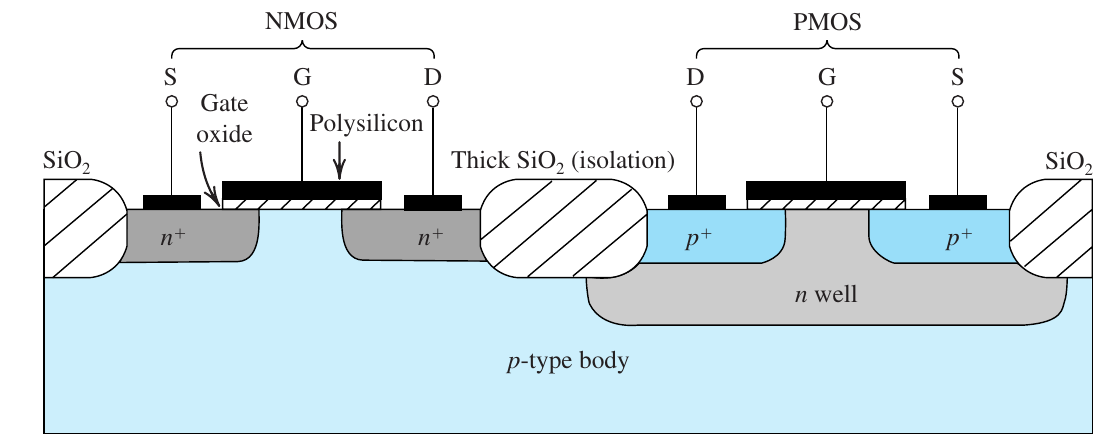
\includegraphics[scale=0.55]{./MOSFET-CMOS-Physical_Structure.png}
  \caption{\nameref*{def:CMOS} Transistor Physical Structure \parencite[p.~264]{sedraTextbook7}}
  \label{fig:MOSFET-Physical_Structure-CMOS}
\end{figure}

\subsection{Operating Regions}\label{subsec:MOSFET_Operating_Regions}
\nameref{def:MOSFET}s operate in one of three regions, based on two different voltages and their relationship.
\begin{enumerate}[noitemsep]
\item \nameref{subsubsec:MOSFET_Cutoff_Region}, $\DCVoltage{GS} < \ThresholdVoltage$
\item \nameref{subsubsec:MOSFET_Triode_Region}, $\DCVoltage{GS} \geq \ThresholdVoltage$ \textbf{and} $\DCVoltage{DS} < \OverdriveVoltage$
\item \nameref{subsubsec:MOSFET_Saturation_Region}, $\DCVoltage{GS} \geq \ThresholdVoltage$ \textbf{and} $\DCVoltage{DS} \geq \OverdriveVoltage$
\end{enumerate}

The current-voltage characteristic of the \nameref{def:NMOS} \nameref{def:MOSFET} is shown in \Cref{fig:MOSFET-Current_Voltage_Characteristic}.

\begin{figure}[h!tbp]
  \centering
  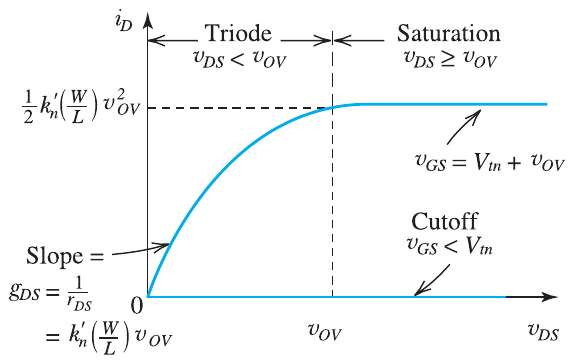
\includegraphics[scale=0.75]{./MOSFET-id_VDS.png}
  \caption{$\ACCurrent{\Drain}$-$\ACVoltage{\Drain\Source}$ \nameref*{def:NMOS} \nameref*{def:MOSFET} Characteristic \parencite[p.~266]{sedraTextbook7}}
  \label{fig:MOSFET-Current_Voltage_Characteristic}
\end{figure}

\subsubsection{Cutoff}\label{subsubsec:MOSFET_Cutoff_Region}
The cutoff region is when the voltage applied at the gate is not enough to make a channel form in the substrate of the \nameref{def:MOSFET}, meaning $\DCVoltage{\Gate\Source} < \ThresholdVoltage$.
Because no channel is formed, no current flows, thus the current is as defined in \Cref{eq:MOSFET_Cutoff_Region-Current}.

\begin{equation}\label{eq:MOSFET_Cutoff_Region-Current}
  \DCCurrent{D} = 0
\end{equation}

\subsubsection{Triode}\label{subsubsec:MOSFET_Triode_Region}
The triode region is formed when the \nameref{def:MOSFET} is turned on ($\ACVoltage{\Gate\Source} \geq \ThresholdVoltage$), and when the channel has not reached its pinchoff point yet ($\ACVoltage{\Drain\Source} < \OverdriveVoltage$).

In short, the two requirements are:
\begin{enumerate}[noitemsep]
\item $\ACVoltage{\Gate\Source} \geq \ThresholdVoltage$
\item $\ACVoltage{\Drain\Source} < \OverdriveVoltage$
\end{enumerate}

\begin{equation}\label{eq:MOSFET_Triode_Region-Current}
  \ACCurrent{\Drain} = k_{n} \left( \OverdriveVoltage - \frac{1}{2} \ACVoltage{\Drain\Source} \right) \ACVoltage{\Drain\Source}
\end{equation}

The \nameref{subsubsec:MOSFET_Triode_Region} has a special case when the drain-source voltage drop is less than the \nameref{def:Overdrive_Voltage}, called the \nameref{par:MOSFET_Linear_Region}.


%%% Local Variables:
%%% mode: latex
%%% TeX-master: "../ECE_311-Engineering_Electronics-Reference_Sheet"
%%% End:
